\documentclass[12pt,a4paper,titlepage]{report}
\renewcommand*{\thefootnote}{[\arabic{footnote}]}
\usepackage{polski}
\usepackage[utf8]{inputenc}
\usepackage{wrapfig} 
\usepackage{graphicx}
\graphicspath{ {figures/} }
\usepackage{array}
\usepackage{bchart}
\usepackage{tikz}
\usepackage{pgf-pie}
\usepackage{natbib}
\usepackage{url}

\author{Damian Folga}

\title{\textbf{Metody przydzielania mandatów wyborczych.}}

\begin{document}

\maketitle
\tableofcontents
\newpage
\chapter{Metoda D'Hondta}
\textbf{Metoda D’Hondta} (również: \textit{Jefferson’s method, Bader-Ofer method}) – metoda stosowana do podziału mandatów w systemach wyborczych opartych na proporcjonalnej reprezentacji z listami partyjnymi. Jej nazwa pochodzi od nazwiska belgijskiego matematyka Victora D’Hondta.
\section{Victor D'Hondt}
Victor D’Hondt\footnote{ Nazwisko D’Hondta jest często niepoprawnie zapisywane jako 'd’Hondt. Przyczyną częstych pomyłek jest wzorowanie się na artykułach holenderskich, gdzie poprawna pisownia pełnego imienia i nazwiska to Victor d’Hondt (mała litera d), a samego nazwiska to D’Hondt (wielka litera D). Jednakże w Belgii obowiązuje zasada zapisu wielką literą w obu przypadkach, czyli poprawny zapis to Victor D’Hondt.} (ur. 20 listopada 1841, zm. 30 maja 1901) – belgijski prawnik, profesor prawa cywilnego i matematyki na uniwersytecie w Gandawie. Najbardziej znany dzięki stworzonej w 1878 roku procedurze podziału mandatów między kandydatów z list partyjnych w wyborach o ordynacji proporcjonalnej, znanej jako metoda D’Hondta.
\newpage
\subsection{Publikacje}
\begin{itemize}
\item{La représentation proportionnelle des partis, 1878}
\item{Système pratique et raisonné de représentation proportionnelle. Bruxelles, 1882.}
\item{Exposé du système pratique de représentation proportionnelle, 1885}
\item{De l'hypothèque spéciale en cas de faillite, 1886}
\item{Concordat préventif, 1890}
\item{Tables de division des nombres 1 à 400 par 1 à 31 et 401 à 1000 par 1 à 13 pour la répartition proportionnelle des sièges en matière électorale avec exposé de la méthode, 1900}
\end{itemize}
\section{Podział mandatów}
W metodzie tej dla każdego komitetu wyborczego, który przekroczył próg wyborczy, obliczane są kolejne ilorazy całkowitej liczby głosów uzyskanych przez dany komitet i kolejnych liczb naturalnych, czyli ilorazy wyborcze. O podziale miejsc pomiędzy komitetami decyduje wielkość obliczonych w ten sposób ilorazów. Można to przedstawić wzorem:

\begin{math}
I_i=\frac{G}{i}
\end{math} \\
gdzie:

\begin{math}
I_i-i
\end{math}
-ty iloraz wyborczy,

\begin{math}
G-
\end{math}
-całkowita liczba głosów oddana na dany komitet w wyborach,

\begin{math}
i-
\end{math}
liczba naturalna,
\begin{math}
i\geq{1}
\end{math}

Tak więc dla każdego komitetu liczba uzyskanych głosów jest dzielona kolejno przez 
\begin{math} 1,2,3,\dots ,n\end{math}. W ten sposób uzyskuje się malejące wielkości 
\begin{math}
I
\end{math}
, które porównywane są następnie z wynikami wszystkich komitetów biorących udział w wyborach i szeregowane w kolejności od największej do najmniejszej. Mandaty przydziela się zgodnie z określoną w ten sposób kolejnością, poczynając od najwyższego wyniku do najniższego, aż do momentu, gdy liczba dostępnych miejsc zostanie wyczerpana.
\newpage
\section{Przykład}
Mamy komitety A, B i C, które otrzymały kolejno 720, 300 i 480 głosów. Do obsadzenia jest 8 mandatów. \\ \\
\textbf{1 krok}: obliczenie ilorazów \\ \\
\begin{table}[h]
\begin{tabular}{|l|l|l|l|} \hline
Dzielnik & Komitet A & Komitet B & Komitet C \\
\hline
1 & 720 (pierwszy mandat) & 300 (czwarty) & 480 (drugi) \\
\hline
2 & 360 (trzeci) & 150 & 240 (szósty) \\
\hline
3 & 240 (piąty) & 100 & 160 (ósmy) \\ 
\hline
4 & 180 (siódmy) & 75 & 120 \\ \hline
5 & 144 & 60 & 96 \\
\hline

\end{tabular}
\caption{Tabela ilorazów uzyskanych przy użyciu metody D'Hondta.}
\end{table}\\ \\
\textbf{2 krok}: ułożenie ilorazów w kolejności malejącej (w nawiasach komitet):
\begin{enumerate}
\item (A) – 720
\item (C) – 480
\item (A) – 360
\item (B) – 300
\item (A) – 240
\item (C) – 240
\item (A) – 180
\item (C) – 160
\end{enumerate} 
itd. \\ \\
\begin{figure} [!htbp]
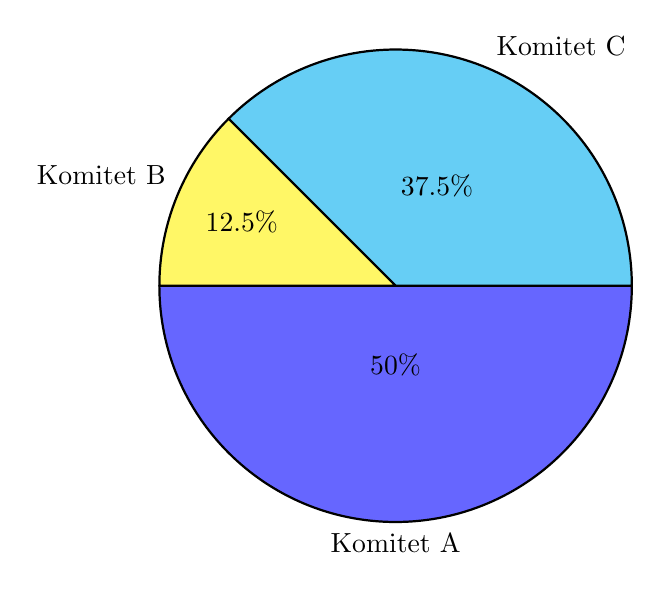
\begin{tikzpicture}
\pie [rotate = 180]
    {50/ Komitet A,
     37.5/Komitet C, 12.5/Komitet B}
\end{tikzpicture}
\caption{Rozkład mandatów uzyskanych poprzez poszczególne komitety przy użyciu metody D'Hondta.}
\end{figure}
W związku z tym, że do rozdzielenia jest 8 mandatów, 4 mandaty otrzymuje komitet A (ilorazy 720, 360, 240 i 180), 1 mandat – komitet B (iloraz 300) oraz 3 mandaty – komitet C (ilorazy 480, 240 i 160). \\ \\
W przypadku gdyby kilka komitetów uzyskało takie same ilorazy stosuje się różne metody dodatkowego szeregowania. W Polsce wybrano następujący sposób – jeżeli kilka list uzyskało ilorazy równe ostatniej liczbie z liczb uszeregowanych w podany sposób, a list tych jest więcej niż mandatów do rozdzielenia, pierwszeństwo mają listy w kolejności ogólnej liczby oddanych na nie głosów. Gdyby na dwie lub więcej list oddano równą liczbę głosów, o pierwszeństwie rozstrzyga liczba obwodów głosowania, w których na daną listę oddano większą liczbę głosów.
\section{Zbliżenie idealnej proporcjonalności}
Doskonała proporcjonalność nie zawsze jest możliwa. Metody reprezentacji proporcjonalnej podchodzą do jej przybliżenia na różne sposoby, które implikują różne koncepcje nieproporcjonalności. Metoda D’Hondta minimalizuje największy współczynnik korzyści, 

\begin{math}max_{k}w_{k}={\frac {m_{k}}{g_{k}}}\end{math}, \\ \
gdzie: \\
\begin{math}w_{k}-\end{math}współczynnik korzyści komitetu
\begin{math}k,\end{math} \\
\begin{math}m_{k}-\end{math}udział mandatów udzielonych do komitetu
\begin{math}k,\end{math} \\
\begin{math} m_{k}\in [0,1],\;\sum\limits _{k}m_{k}=1,\end{math} \\
\begin{math}g_{k}-\end{math}udział głosów oddanych na komitet
\begin{math}k,\end{math} w wyborach,\\
\begin{math} g_{k}\in [0,1],\;\sum\limits_{k} g_{k}=1.\end{math}\footnote{André Sainte-Laguë. La représentation Proportionnelle et la méthode des moindres carrés. „Annales scientifiques de l’École Normale Supérieure”. 27, 1910. l’École Normale Supérieure (fr.).} \\
Metoda D’Hondta dzieli głosy na dokładnie proporcjonalnie reprezentowane i niereprezentowane, minimalizując udział niereprezentowanych głosów 

\begin{math}\pi ^{*}=1-{\frac {1}{\max _{k}w_{k}}}\end{math}\footnote[2]{Juraj Medzihorsky. Rethinking the D’Hondt method. „Political Research Exchange”. 1(1), 2019. Taylor \& Francis (ang.).} \\
Niereprezentowany udział głosów komitetu jest
\begin{math} n_{k}=g_{k}-(1-\pi ^{*})m_{k},\;n_{k}\in [0,g_{k}],\sum _{k}\,n_{k}=\pi ^{*}\end{math}\footnotemark[2]
 \\ \\
Przy minimalizacji ogólnej liczby niereprezentowanych głosów metoda D’Hondta bierze pod uwagę tylko największy współczynnik korzyści. Jeśli do oceny proporcjonalności stosuje się współczynnik korzyści, wynika to z tego że metoda D’Hondta faworyzuje duże ugrupowania w większym stopniu niż druga spośród najpopularniejszych metod przeliczania głosów – metoda Sainte-Laguë.
\newpage
\section{Stosowanie}
Metoda D’Hondta jest najczęściej stosowaną metodą reprezentacji proporcjonalnej w wyborach do parlamentów narodowych\footnote[3]{Nils-Christian Bormann and Matt Golder. Democratic electoral systems around the world, 1946--2011. „Electoral Studies”. 32(2), 2013. Elsevier (ang.).}. Stosuje się ją przy podziale mandatów w wyborach parlamentarnych m.in. w Austrii, Finlandii, Izraelu, Holandii i Hiszpanii. W Polsce stosowano ją m.in. w parlamentarnych ordynacjach wyborczych II Rzeczypospolitej (do 1935 r.), a także w III Rzeczypospolitej (z wyłączeniem wyborów w 1991 r. oraz wyborów w 2001 r.) przy podziale mandatów do Sejmu oraz w wyborach samorządowych (do rad gmin powyżej 20 000 mieszkańców\footnote[4]{ Zgodnie z art. 373. § 2 Kodeksu Wyborczego, przez mieszkańców należy rozumieć dorosłych wyborców zamieszkałych na obszarze działania danej rady, ujętych w stałym rejestrze wyborców na koniec roku poprzedzającego rok, w którym wybory mają być przeprowadzone.}, rad powiatów oraz sejmików województw).

W Izraelu metoda ta jest w użyciu od 1973, przy czym znana jest pod nazwą Bader-Ofer method od nazwisk parlamentarzystów, którzy zaproponowali jej wprowadzenie (Jochanan Bader i Awraham Ofer)\footnote[5]{The Distribution of Seats Among the Lists}.
\newpage
\chapter{Metoda Sainte-Laguë}
\textbf{Metoda Sainte-Laguë} – metoda stosowana do podziału mandatów w systemach wyborczych opartych na proporcjonalnej reprezentacji z listami partyjnymi. Jej nazwa pochodzi od nazwiska francuskiego matematyka André Sainte-Laguë.

Metoda polega na znalezieniu największych, kolejno po sobie następujących ilorazów z liczby uzyskanych głosów. Podziału dokonuje się, dzieląc liczbę głosów przypadających każdemu komitetowi wyborczemu przez kolejne liczby nieparzyste: 1, 3, 5, 7, itd., a następnie z tak obliczonych ilorazów dla wszystkich komitetów wybieranych jest tyle największych, ile jest mandatów do obsadzenia.

Istnieją różne odmiany tej metody. Niekiedy pomija się pierwszy dzielnik, dzieląc liczbę uzyskanych głosów kolejno przez 3, 5, 7 itd. Popularną modyfikacją jest zastąpienie pierwszego dzielnika 1 przez 1,4 , co sprzyja ugrupowaniom większym – system ten znany jest jako zmodyfikowana metoda Sainte-Laguë.
\section{Wykorzystywanie}
Metoda Sainte-Laguë jest stosowana m.in. w systemach wyborczych w Nowej Zelandii, Norwegii, Szwecji, Bośni i Hercegowinie, Łotwie oraz Kosowie, a od 2009 roku również w Niemczech. Jest stosowana, także w Niemczech w wyborach do Landtagów: Badenii-Wirtembergii, Hamburga, Bremy, Nadrenii Północnej-Westfalii oraz Nadrenii-Palatynatu. Użyto jej również w wyborach w Boliwii w 1993 roku, wyborach do Rady Legislacyjnej Autonomii Palestyńskiej w 2006 roku i w wyborach parlamentarnych w Nepalu w 2008 roku. Zastosowano ją także (w wersji zmodyfikowanej) w Polsce podczas wyborów parlamentarnych w 1991 roku oraz w wyborach do rad gmin (w gminach liczących powyżej 20 tys. mieszkańców) w 1990 i 1994 r.

Metoda Sainte-Laguë generuje wyniki lepiej odzwierciedlające poglądy wyborców, podczas gdy metoda D’Hondta sprzyja większym partiom.
\section{Przykład}
Mamy komitety A, B oraz C, które otrzymały kolejno 720, 300 i 480 głosów, do obsadzenia jest 8 mandatów. \\
\textbf{1 krok}: obliczenie ilorazów \\ \\
\begin{table}[]
\begin{tabular}{|l|l|l|l|} \hline
Dzielnik & Komitet A & Komitet B & Komitet C \\
\hline
1 & 720 (pierwszy mandat) & 300 (trzeci) & 480 (drugi) \\
\hline
3 & 240 (czwarty) & 100 (ósmy) & 160 (piąty) \\
\hline
5 & 144 (szósty) & 60 & 96 \\ 
\hline
7 & 103 (siódmy) & 43 & 69 \\
\hline

\end{tabular}
\caption{Tabela ilorazów uzyskanych przy użyciu metody Sainte-Laguë'a}
\end{table}\\ \\
\textbf{2 krok}: ułożenie ilorazów w kolejności malejącej (w nawiasach komitet):
\begin{enumerate}
\item (A) – 720
\item (C) – 480
\item (B) – 300
\item (A) – 240
\item (C) – 160
\item (A) – 144
\item (A) – 103
\item (B) – 100
\end{enumerate} 
itd. 
\begin{figure} [!htbp]
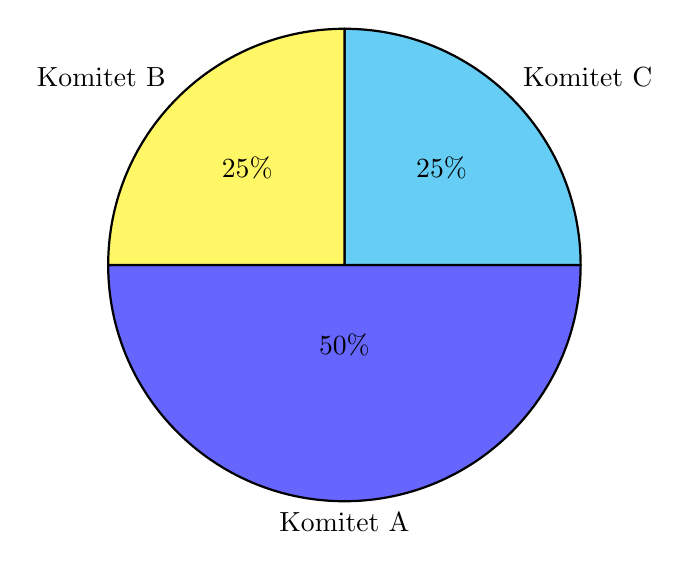
\begin{tikzpicture}
\pie [rotate = 180]
    {50/ Komitet A,
     25/Komitet C, 25/Komitet B}
\end{tikzpicture}
\caption{Rozkład mandatów uzyskanych poprzez poszczególne komitety przy użyciu metody  Sainte-Laguë'a.}
\end{figure}
\newpage
\section{Implementacja w języku Python}
Liczba mandatów może być obliczona przez następujący kod w języku Python: 
\begin{verbatim}
V = [liczba głosów dla A,liczba głosów dla B,liczba głosów dla C]
s = [0,0,0]

for j in range(liczba mandatów):
    imax = 0
    for i in range(len(V)):
      if (V[i]/(2 * s[i] + 1)) > (V[imax]/(2 * s[imax] + 1)):
        imax = i

    s[imax] = s[imax] + 1

print s
\end{verbatim}
\newpage
\chapter{Metoda Hare’a-Niemeyera}
\textbf{Metoda Hare’a-Niemeyera} – metoda stosowana do podziału mandatów w systemach wyborczych opartych na proporcjonalnej reprezentacji z listami partyjnymi, powstała na skutek modyfikacji metody Hare’a przez niemieckiego matematyka Horsta Niemeyera. Nazywana jest także metodą największych reszt\footnotemark[1] lub matematycznej proporcji.
Liczbę uzyskanych mandatów oblicza się za pomocą wzoru\footnotemark[1]:

\begin{math} Q={\frac {V_{1}\cdot S}{V_{t}}}=X,...\end{math}\\
gdzie:

\begin{math}Q-\end{math} liczba uzyskanych przez daną listę mandatów,

\begin{math}V_1-\end{math} liczba ważnie oddanych głosów na daną listę w okręgu wyborczym,

\begin{math}S-\end{math} liczba mandatów do obsadzenia w danym okręgu wyborczym,

\begin{math}V_t-\end{math} łączna liczba głosów oddanych w danym okręgu wyborczym,

\begin{math}X,...-\end{math} wynik dzielenia, np. 1,38. \\
Liczba \textbf{X} przed przecinkiem oznacza liczbę mandatów przypadających w okręgu wyborczym danej liście. Jeżeli w odniesieniu do wszystkich list okręgowych nie zostaną rozdzielone wszystkie mandaty, to pozostałe mandaty przydziela się tym listom, dla których wyliczone ilorazy wykazują kolejno najwyższe wartości po przecinku, np. 0,39; 0,27; 0,05. Stosuje się wtedy zasadę największej reszty\footnote[1]{Metoda Hare-Niemeyer'a - Algorytmy i Struktury Danych, www.algorytm.org [dostęp 2019-10-23].}.

W Polsce tę metodę stosowano przy ustalaniu wyników w wyborach do Sejmu w 1991 roku\footnote[2]{www.NAUKA.uj.edu.pl - Nauka - Uniwersytet Jagielloński, nauka.uj.edu.pl [dostęp 2019-10-23].}.\cite{wiki:3}
\newpage
\section{Przykład}
Mamy komitety A, B oraz C, które otrzymały kolejno 720, 300 i 480 głosów, do obsadzenia jest 8 mandatów. Według powyższego wzoru, obliczamy współczynniki dla poszczególnych komitetów:\\
\begin{itemize}
\item{\begin{math} A-{\frac {720\cdot 8}{720+300+480}}=3{,}84,\end{math}}\
\item{\begin{math} B-{\frac {300\cdot 8}{720+300+480}}=1{,}6, \end{math}}\
\item{\begin{math} C-{\frac {480\cdot 8}{720+300+480}}=2{,}56.\end{math}}
\end{itemize}
Zgodnie z liczbami przed przecinkiem, 3 mandaty uzyskuje komitet A, jeden komitet B, a dwa komitet C. Pozostałe dwa mandaty zostają rozdzielone kolejno komitetom o najwyższej wartości po przecinku, czyli A, następnie B. Ostatecznie komitet A uzyskuje 4 mandaty, a komitety B i C po dwa.
\begin{figure} [!htbp]
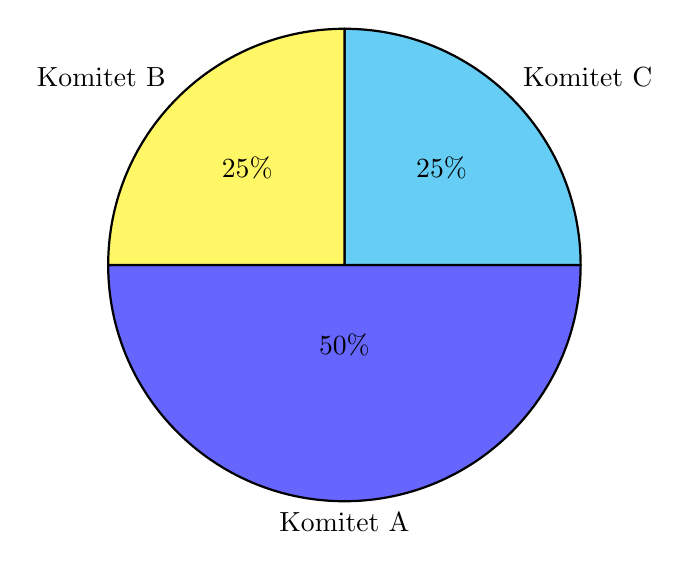
\begin{tikzpicture}
\pie [rotate = 180]
    {50/ Komitet A,
     25/Komitet C, 25/Komitet B}
\end{tikzpicture}
\caption{Rozkład mandatów uzyskanych poprzez poszczególne komitety przy użyciu metody  Hare-Niemeyer'a.}
\end{figure}
\newpage
	\addcontentsline{toc}{section}{Spis rysunków}
	\listoffigures
	\addcontentsline{toc}{section}{Spis tabel}
	\listoftables
\newpage
\bibliographystyle{plain}
\bibliography{Bibliografia}
\end{document}
